\documentclass[11pt,a4paper]{article}

\usepackage[utf8]{inputenc}
\usepackage[english]{babel}
\usepackage[T1]{fontenc}
\usepackage{listings}
\usepackage{amsmath,amssymb,amsfonts}
\usepackage{graphicx}

\title{Individual Compiler Assignment - w2}
\author{Jonas Brunsgaard}

\begin{document}
\maketitle

\section{Writing Context-Free Grammars}

\subsection{Define a CFG for $\{a^i b^j c^i | a, b, c\in \sum; i, j > 0\}$}
Below I have defined the context free grammar.
\begin{eqnarray*}
    S & \rightarrow & aTc \\
    T & \rightarrow & S \\
    T & \rightarrow & R \\
    R & \rightarrow & cR \\
    R & \rightarrow & c
\end{eqnarray*}

\subsection{Show the left-most derivation of the word 'aabbcc'}
Below you find the leftmost derivation of the string

\begin{align*}
    \, & S\\
    \Rightarrow\, & a\underline{T}c\\
    \Rightarrow\, & aa\underline{T}cc\\
    \Rightarrow\, & aa\underline{R}cc\\
    \Rightarrow\, & aab\underline{R}cc\\
    \Rightarrow\, & aabbcc
\end{align*}

\section{LL(1)-Parser Construction}
\subsection{Eliminating left-recursion and left-factorise the grammar}
We eliminate left recursion
$$
\begin{array}{lcl}
    S & \rightarrow & \mathrm{id}\\
    S & \rightarrow & \mathrm{id[} E \mathrm{]}\\
    E & \rightarrow & SE^{*}\\
    E^{*} & \rightarrow & \varepsilon\\
    E^{*} & \rightarrow & \mathrm{,}E
\end{array}
$$
and follow up with left-factorisation
$$
\begin{array}{lcl}
    S & \rightarrow & \mathrm{id}S^{*}\\
    S^{*} & \rightarrow & \varepsilon\\
    S^{*} & \rightarrow & \mathrm{[} E \mathrm{]}\\
    E & \rightarrow & SE^{*}\\
    E^{*} & \rightarrow & \varepsilon\\
    E^{*} & \rightarrow & \mathrm{,}E
\end{array}
$$
\subsection{Calculate First sets}

First we find if terminals and nonterminals are \emph{nullable}.
\begin{center}
\begin{tabular}{c||c|c|c}
Right-hand side & Init & First Iter & Sec Iter\tabularnewline
\hline 
\hline 
$\mathrm{id}$ & \emph{false} & \emph{false} & \emph{false}\tabularnewline
\hline 
$\varepsilon$ & \emph{false} & \emph{true} & \emph{true}\tabularnewline
\hline 
$[E\mathrm{\mathrm{]}}$ & \emph{false} & \emph{false} & \emph{false}\tabularnewline
\hline 
$SE^{*}$ & \emph{false} & \emph{false} & \emph{false}\tabularnewline
\hline 
$\mathrm{,}E$ & \emph{false} & \emph{false} & \emph{false}\tabularnewline
\hline 
Nonterminal & \multicolumn{1}{c}{} & \multicolumn{1}{c}{} & \tabularnewline
\hline 
$S$ & \emph{false} & \emph{false} & \emph{false}\tabularnewline
\hline 
$S^{*}$ & \emph{false} & \emph{true} & \emph{true}\tabularnewline
\hline 
$E$ & \emph{false} & \emph{false} & \emph{false}\tabularnewline
\hline 
$E^{*}$ & \emph{false} & \emph{true} & \emph{true}\tabularnewline
\end{tabular}
\end{center}
Then we calculate \emph{FIRST}:

\begin{center}
\begin{tabular}{c||c|c|c}
Right-hand side & Init & First Iter & Sec Iter\tabularnewline
\hline 
\hline 
$\mathrm{id}$ & \emph{$\emptyset$} & $\{\mathrm{id}\}$ & $\{\mathrm{id}\}$\tabularnewline
\hline 
$\varepsilon$ & \emph{$\emptyset$} & \emph{$\emptyset$} & \emph{$\emptyset$}\tabularnewline
\hline 
$[E\mathrm{\mathrm{]}}$ & \emph{$\emptyset$} & $\{[\}$ & $\{[\}$\tabularnewline
\hline 
$SE^{*}$ & \emph{$\emptyset$} & $\{\mathrm{id}\}$ & $\{\mathrm{id}\}$\tabularnewline
\hline 
$\mathrm{,}E$ & \emph{$\emptyset$} & $\{,\}$ & $\{,\}$\tabularnewline
\hline 
Nonterminal & \multicolumn{1}{c}{} & \multicolumn{1}{c}{} & \tabularnewline
\hline 
$S$ & \emph{$\emptyset$} & $\{\mathrm{id}\}$ & $\{\mathrm{id}\}$\tabularnewline
\hline 
$S^{*}$ & \emph{$\emptyset$} & $\{[\}$ & $\{[\}$\tabularnewline
\hline 
$E$ & \emph{$\emptyset$} & $\{\mathrm{id}\}$ & $\{\mathrm{id}\}$\tabularnewline
\hline 
$E^{*}$ & \emph{$\emptyset$} & $\{,\}$ & $\{,\}$\tabularnewline
\end{tabular}
\end{center}

\subsection{Calculate Follow sets for all nonterminals}
By following the procedure on page 59 in the book, we find the following table.
\begin{center}
\begin{tabular}{ll}
\hline 
Production & Constraints\tabularnewline
\hline 
$S'\rightarrow S\$$ & $\{\$\}\subseteq FOLLOW(S)$\tabularnewline
$S\rightarrow\mathrm{id}S^{*}$ & $FOLLOW(S)\subseteq FOLLOW(S^{*})$\tabularnewline
$S^{*}\rightarrow\varepsilon$ & \tabularnewline
$S^{*}\rightarrow[E]$ & $\{\mathrm{]}\}\subseteq FOLLOW(E)$\tabularnewline
$E\rightarrow SE^{*}$ & %
\begin{minipage}[t]{0.5\columnwidth}%
$\{\mathrm{,}\}\subseteq FOLLOW(S)$ \\
$FOLLOW(E)\subseteq FOLLOW(S)$ \\
$FOLLOW(E)\subseteq FOLLOW(E^{*})$%
\end{minipage}\tabularnewline
$E^{*}\rightarrow\varepsilon$ & \tabularnewline
$E^{*}\rightarrow\mathrm{,}E$ & $FOLLOW(E^{*})\subseteq FOLLOW(E)$\tabularnewline
\hline
\end{tabular}
\end{center}
In the table above I have used the $FIRST$-sets we calcualted earlier, and thus they are shown as explicit terminals.

We first use the constraints $ \{\$\} \subseteq FOLLOW(S)$ and constraints
of the form $FIRST(\dots)\subseteq FOLLOW(\dots)$ to get the initial sets.
Note, that in the following i will use the word ``komma'' to refer to the
terminal ``,''. The reason be that the symbol ``," are used as seperator, when
describing a set.
\begin{eqnarray*}
    FOLLOW(S)       & \supseteq & \{\mathrm{komma, \$} \} \\
    FOLLOW(S^{*})   & \supseteq & \{\emptyset\} \\
    FOLLOW(E)       & \supseteq & \{\mathrm{]}\} \\
    FOLLOW(E^{*})   & \supseteq & \{\emptyset\}
\end{eqnarray*}
and then use the constrains on the form $FOLLOW(\dots)\subseteq FOLLOW(\dots)$. After first iteration:
\begin{eqnarray*}
    FOLLOW(S)       & \supseteq & \{\mathrm{komma,\$]}\} \\
    FOLLOW(S^{*})   & \supseteq & \{\mathrm{komma, \$}\} \\
    FOLLOW(E)       & \supseteq & \{\mathrm{]}\} \\
    FOLLOW(E^{*})   & \supseteq & \{\mathrm{]}\}
\end{eqnarray*}
second iteration:
\begin{eqnarray*}
    FOLLOW(S)       & \supseteq & \{\mathrm{komma,\$]}\} \\
    FOLLOW(S^{*})   & \supseteq & \{\mathrm{komma,\$]}\} \\
    FOLLOW(E)       & \supseteq & \{\mathrm{]}\} \\
    FOLLOW(E^{*})   & \supseteq & \{\mathrm{]}\}
\end{eqnarray*}
and the third iteration, nothing has changed, so the final result is
\begin{eqnarray*}
    FOLLOW(S)       & =         & \{\mathrm{komma,\$]}\} \\
    FOLLOW(S^{*})   & =         & \{\mathrm{komma,\$]}\} \\
    FOLLOW(E)       & =         & \{\mathrm{]}\} \\
    FOLLOW(E^{*})   & =         & \{\mathrm{]}\}
\end{eqnarray*}
\subsection{Look-aheads sets and pseudo code}
From the lecture slides the look ahead set is defined as
$$la(X\rightarrow\alpha)=
\begin{cases}
    FIRST(\alpha)\cup FOLLOW(X) & \textrm{, if }NULLABLE(\alpha)\\
    FIRST(\alpha)               & \textrm{, otherwise}
\end{cases}$$
Below the lookahead sets for our productions are shown.
$$
\begin{array}{lcl}
    LA(S' \rightarrow S\$)           & = &      \{\mathrm{id}\} \\
    LA(S \rightarrow \mathrm{id}S^{*})    & = &      \{\mathrm{id}\} \\
    LA(S^{*} \rightarrow \varepsilon)& = &      \{\emptyset\} \\
    LA(S^{*} \rightarrow \mathrm{[}E\mathrm{]})& = &      \{\mathrm{[}\} \\
    LA(E \rightarrow SE^{*})         & = &      \{\mathrm{id}\} \\
    LA(E^{*} \rightarrow \varepsilon)& = &      \{\emptyset\} \\
    LA(E^{*} \rightarrow \mathrm{komma}E)& = &  \{\mathrm{komma}\} \\
\end{array}
$$
We now build our pseudo code for the parser:
\begin{lstlisting}
function parseS' () = 
    if next = 'id' 
    then parseT(); match('\$')
    else reportError()

function parseS () =
    if next = 'id'
    then match('id'); parseS*()
    else reportError()

function parseS* () =
    if next = '\$'
    then (* do nothing *)
    else if next = '['
         then match('['); parseE(); match(']')
         else reportError()

function parseE () =
    if next = 'id'
    then parseS(); parseE*()
    else reportError()

function parseE* () =
    if next = '\$'
    then (* do nothing *)
    else if next = ','
         then match(','); parseE();
         else reportError()

\end{lstlisting}
\section{SLR Parser Construction}
First we produce NFA's for the right hand side of every production.


\begin{center}
    \begin{tabular}{l|l}
    Production          & NFA\\ \hline
        \raisebox{-7pt}{$S \rightarrow E$}                        & \raisebox{-15pt}{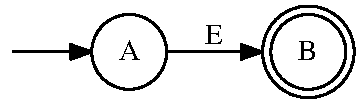
\includegraphics[height=22pt]{nfa-p0.pdf}} \\
        \raisebox{-7pt}{$E \rightarrow \mathrm{a}$}               & \raisebox{-15pt}{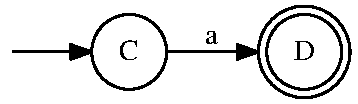
\includegraphics[height=22pt]{nfa-p1.pdf}} \\
        \raisebox{-7pt}{$E \rightarrow \mathrm{a(} E \mathrm{)}$} & \raisebox{-15pt}{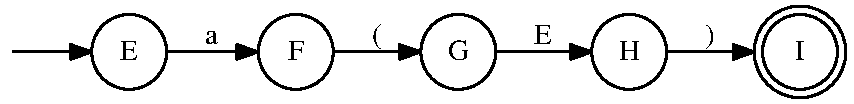
\includegraphics[height=22pt]{nfa-p2.pdf}} \\
        \raisebox{-7pt}{$E \rightarrow E \mathrm{\&a}$}          & \raisebox{-15pt}{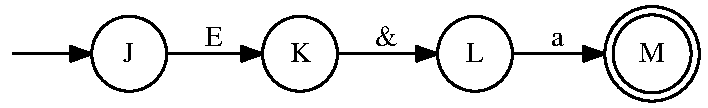
\includegraphics[height=22pt]{nfa-p3.pdf}}
    \end{tabular}
\end{center}
If an NFA state $s$ has an outgoing transition on nonterminal $N$ we add a
lambda transition from $s$ to the starting states of the NFAs for the rhs of
the productions for $N$.
\begin{center}
    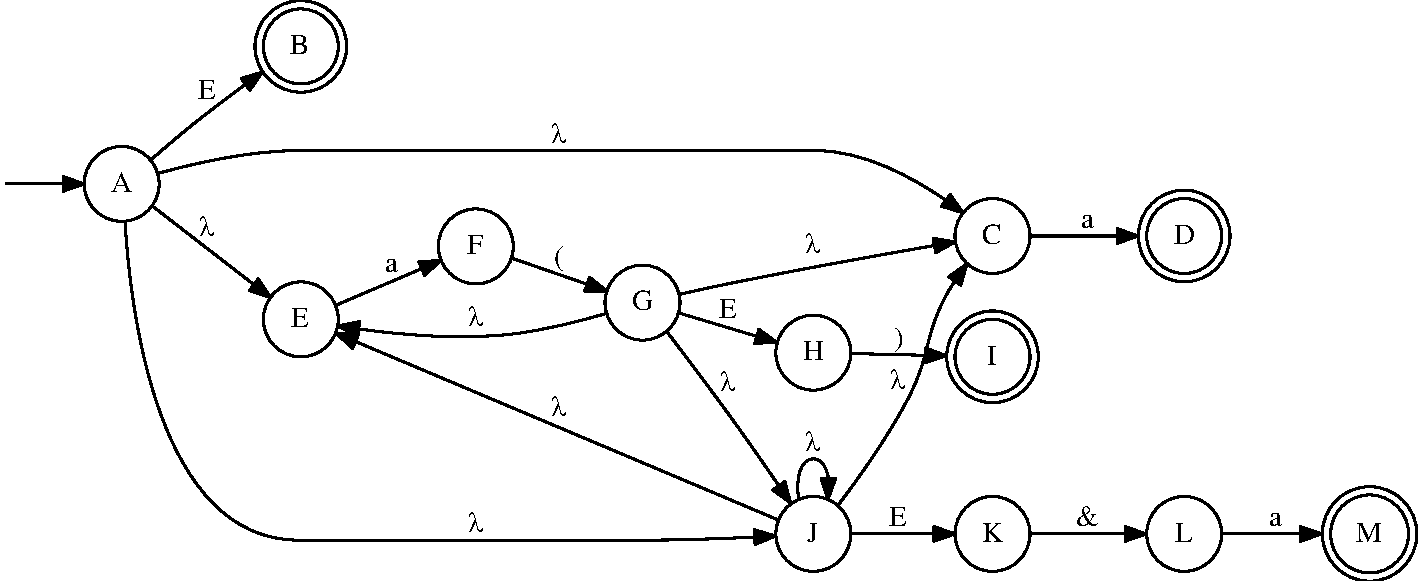
\includegraphics[width=0.9\textwidth]{nfa-combined.pdf}
\end{center}
Then  we convert the combined  NFA to a DFA.
$$
\begin{array}{lcl}
    \hat{\lambda} (A) & = & \{A,C,E,J\} = s_{0}\\
    move(s_{0},a)   & = & \hat{\lambda} (\{D, F \})     = \{D, F\}          = s_{1} \\
    move(s_{0},E)   & = & \hat{\lambda} (\{B, K \})     = \{B, K\}          = s_{2} \\
    move(s_{1},()   & = & \hat{\lambda} (\{G \})        = \{G, C, E, J\}    = s_{3} \\
    move(s_{2},\&)  & = & \hat{\lambda} (\{L \})        = \{L \}            = s_{4} \\
    move(s_{3},a)   & = & \hat{\lambda} (\{D, F\})      = \{D , F \}        = s_{1} \\
    move(s_{3},E)   & = & \hat{\lambda} (\{K, H \})     = \{K, H\}          = s_{5} \\
    move(s_{4},a)   & = & \hat{\lambda} (\{M \})        = \{M\}             = s_{6} \\
    move(s_{5},))   & = & \hat{\lambda} (\{I \})        = \{I\}             = s_{7} \\
    move(s_{5},\&)  & = & \hat{\lambda} (\{L \})        = \{L\}             = s_{4}
\end{array}
$$
Now we are able to build the initial cross index table
\begin{center}
    \begin{tabular}{c|c|c c c c|c}
        DFA state   & NFA states    & a     & (     & )     & $\&$  & $E$  \\ \hline
        0           & A,C,E,J       & s1    &       &       &       & g2  \\      
        1           & D,F           &       & s3    &       &       & \\      
        2           & K,B           &       &       &       & s4    & \\      
        3           & G,C,E,J       & s1    &       &       &       & g5 \\      
        4           & L             & s6    &       &       &       & \\      
        5           & H,K           &       &       & s7    & s4    & \\      
        6           & M             &       &       &       &       & \\      
        7           & I             &       &       &       &       & \\      
    \end{tabular}
\end{center}
The follow set for the production $E$ and $S$, has been computed 
\begin{center}
    $$
    \begin{array}{lcl}
        FOLLOW(S) &=& \{\$\} \\
        FOLLOW(E) &=& \{\$,),\&\}
    \end{array}
    $$
\end{center}
and used to determine wheather we shift or reduce. Below the finale table can be seen.
\begin{center}
    \begin{tabular}{c|c c c c c|c}
        DFA state   & a     & (     & )     & $\&$  & $\$$  & $E$  \\ \hline
        0           & s1    &       &       &       &       & g2  \\
        1           &       & s3    & r1    & r1    & r1    & \\
        2           &       &       &       & s4    & a     & \\
        3           & s1    &       &       &       &       & g5 \\
        4           & s6    &       &       &       &       & \\
        5           &       &       & s7    & s4    &       & \\
        6           &       &       & r3    & r3    & r3    & \\
        7           &       &       & r2    & r2    & r2    & \\
    \end{tabular}
\end{center}
\subsection{Parsing the input "a(a\&a)"}
\begin{center}
    \begin{tabular}{r|l|l}
        Input   & stack     & action \\ \hline
        a(a\&a)  & 0        & s1 \\
         (a\&a)  & 01       & s3 \\
          a\&a)  & 0131     & s1 \\
           \&a)  & 0135     & r1($E\rightarrow a$); g5 \\
           \&a)  & 01354    & s4 \\
              )  & 013546   & r3($E \rightarrow E\mathrm{\&a}$); g5 \\
              )  & 0135     & s7 \\
             \$  & 10357    & r2($E \rightarrow \mathrm{a(}E\mathrm{)}$); g2 \\
             \$  & 02       & a 
    \end{tabular}
\end{center}
\subsection{Build a parser in mosmlyac}
After compiling the .grm file, it is clear from the output file, that mosmlyac are using SLR parsing.
\begin{center}
    \begin{tabular}{c|ccccccc|ccc}
        DFA state    & a   & (     & )     & $\&$  & '\textbackslash001'   & EOF   & $\%end$   & $\%entry$  & $S$   & $E$ \\ \hline
         0           &     &       &       &       & s1    &       &           & g2         &       & \\      
         1           & s3  &       &       &       &       &       &           &            & g4    & g5 \\      
         2           &     &       &       &       &       &       & a         &            &       & \\      
         3           &     & s6    & r2    & r2    &       & r2    &           &            &       & \\      
         4           & r5  & r5    & r5    & r5    & r5    & r5    & r5        &            &       & \\      
         5           &     &       &       & s7    &       & s8    &           &            &       & \\      
         6           & s3  &       &       &       &       &       &           &            &       & g9\\      
         7           & s10 &       &       &       &       &       &           &            &       & \\      
         8           & r1  & r1    & r1    & r1    & r1    & r1    & r1        &            &       & \\      
         9           &     &       & s11   & s7    &       &       &           &            &       & \\      
        10           & r4  & r4    & r4    & r4    & r4    & r4    & r4        &            &       & \\      
        11           & r3  & r3    & r3    & r3    & r3    & r3    & r3        &            &       & \\      
    \end{tabular}
\end{center}
We can see that the two tables are not that different and i try to parse the string '\textbackslash001a(a\&a)EOF'
\begin{center}
    \begin{tabular}{r|l|l}
        Input    & stack             & action \\ \hline
  '\textbackslash001'a(a\&a)  & 0                & s1 \\
        a(a\&a)  & 0 1              & s3 \\
         (a\&a)  & 0 1 3            & s6 \\
          a\&a)  & 0 1 3 6          & s3 \\
           \&a)  & 0 1 3 6 3        & r2; g9 \\
           \&a)  & 0 1 3 6 9        & s7 \\
             a)  & 0 1 3 6 9 7      & s10 \\
              )  & 0 1 3 6 9 7 10   & r4; g9 \\
              )  & 0 1 3 6 9        & s11 \\
            EOF  & 0 1 3 6 9 11     & r3; g5 \\
            EOF  & 0 1 5            & s8 \\
             \$  & 0 1 5 8          & r1; g4 \\
             \$  & 0 1 4            & r5; g2 \\
             \$  & 0 2              & 1 \\
    \end{tabular}
\end{center}
The parser generator introduces some new terminals and some nonterminale e.g. \%entry and \%end, but overall the handmade SLR table and the parsergenerated SLR table are not that different.
\end{document}
